\documentclass[../../time_series_notes.tex]{subfiles}
\begin{document}
%%%%%%%%%%%%%%%%%%%%%%%%%%%%%%
\section{Measures of Dependence}
A complete description of a time series where we observe $n$ variables at the time instances $t_{1}, t_{2}, \ldots, t_{n}$ can be given by the joint cumulative distribution function (with constants $c_{1}, c_{2}, \ldots, c_{n}$)
\begin{align*}
    F(x_{1}, x_{2}, \ldots, x_{n}) = P(x_{1} \leq c_{1}, x_{2} \leq c_{2}, \ldots x_{n} \leq c_{n})
\end{align*}
But this is rarely easy to calculate and takes a tractable form when the variables are jointly normal. The marginal distributions in general are
\begin{align*}
    F_{t}(x) &= P(x_{t} \leq x)\\
    f_{t}(x) &= \frac{\partial F_{t}(x)}{\partial x}
\end{align*}


%%%%%%%%%%%%%%%%%%%%
\subsection{Mean Function} \label{mean_fun}
The mean function is similar to the usual definition of the expected value
\begin{align*}
    \mu_{xt} = E[x_{t}] =  \int_{-\inf}^{\inf} x f_{t}(x) dx
\end{align*}

\textbf{Smoothing a series does not change it's mean}.
\begin{align*}
    v_{t} &= \frac{1}{3}(x_{t-1} + x_{t} + x_{t+1})\\
    E[v_{t}] &= \frac{1}{3}(3E[x_{t}]) = E[x_{t}]
\end{align*}

Consider the random walk defined earlier with noise $w_{t}$ and also consider it's mean
\begin{align*}
    \mu_{t} = \delta t + \sum_{t} w_{t}\\
    E[\mu_{t}] = \delta t
\end{align*}
since the mean of noise is zero. Thus, at any given instance, the walk is expected to lie on the straight line $\delta t$ with some noise added on top of it.\newline
In a similar manner, laying a noise on top of the signal will not change the mean value because of the additive nature. The mean of the noise will become zero and the mean of the new signal will be same as the mean of the original signal.


%%%%%%%%%%%%%%%%%%%%
\subsection{Autocovariance Function}
For any two time points $s$ and $t$,
\begin{align*}
    \gamma_{x}(s, t) = E[(x_{s} - \mu_{s})(x_{t} - \mu_{t})]
\end{align*}
which is similar to the covariance between the two points. Note that the function is symmetric and $\gamma_{x}(s, t) = \gamma_{x}(t, s)$. The prefix auto before covariance distinguishes it from covariance used in the context of random variables.\newline

The autocovariance is a measure of linear dependence between two points of the same time series. \textbf{For very smooth series, the autcovariance tends to take large values while for choppy series, it tends to take very small values}.\newline

Consider the example of a white noise series. We know that any nearby points are not correlated with one another. The same will hold with the autocovariance values as well. It will be zero when $s \neq t$ and $\sigma_{w}^{2}$ when $s = t$.\newline

\subsection{Covariance of Linear Combinations}
For linear combinations of random variables $X_{i}$ and $Y_{j}$, the following holds
\begin{align*}
    U &= \sum_{i=1}^{n} a_{i} X_{i}\\
    V &= \sum_{j=1}^{m} b_{j} Y_{j}\\
    Cov(U,V) &= \sum_{i=1}^{n} \sum_{j=1}^{m} a_{i} b_{j} Cov(X_{i}, Y_{j})\\
    Var(U) &= Cov(U,U)
\end{align*}
As an example, consider the covariance calculation for the moving averages of white noise defined as
\begin{align*}
    v_{t} &= \frac{1}{3}(w_{t-1} + w_{t} + w_{t+1})\\
    Cov(t, t) &= \frac{1}{9}(Cov(w_{t-1}, w_{t-1}) + Cov(w_{t}, w_{t}) + Cov(w_{t+1}, w_{t+1}))\\
    &= \frac{3}{9} \sigma_{w}^{2}
\end{align*}
because the covariance between any two different points in the white noise time series is zero and the covariance of a point with itself will be the variance.\newline
Continuing the calculation for different time points
\begin{align*}
    Cov(t+1, t) &= Cov(\frac{1}{3}(w_{t} + w_{t+1} + w_{t+2}), \frac{1}{3}(w_{t-1} + w_{t} + w_{t+1}))\\
    &= \frac{1}{9}(Cov(w_{t}, w_{t}) + Cov(w_{t+1}, w_{t+1}))\\
    &= \frac{2}{9}\sigma_{w}^{2}
\end{align*}
If we continue the calculation, we will observe that the covariance diminishes once we calculate the value between two time points which are more than three time steps apart. This should be the case since then the two points for which the covariance is being calculated will not have any overlapping terms.
\begin{align*}
    % \hypertarget{ma_noise_cov}{\gamma(s,t)} = \begin{cases} \frac{3}{9}\sigma_{w}^{2} &\mbox{$s = t$},\\
    \gamma(s,t) = \begin{cases} \frac{3}{9}\sigma_{w}^{2} &\mbox{$s = t$},\\
                                \frac{2}{9}\sigma_{w}^{2} &\mbox{$\lvert s - t \rvert = 1$}\\
                                \frac{1}{9}\sigma_{w}^{2} &\mbox{$\lvert s - t \rvert = 2$}\\
                                0 &\mbox{otherwise} \end{cases} \numberthiseqn\label{eq:gamma_ma}
\end{align*}


%%%%%%%%%%%%%%%%%%%%
\subsection{Autocorrelation Function (ACF)}
This measure tries to bring the auto correlation value in the range of $[-1,1]$
\begin{align*}
    \rho(s,t) = \frac{\gamma_{x}(s,t)}{\sqrt{\gamma_{x}(s,s) \gamma_{x}(t,t)}}
\end{align*}
With the \emph{Cauchy Schwarz Inequality}, the numerator is always less than or equal to the denominator, bringing the value in the range $[-1,1]$. This value also gives a rough measure of the ability to forecast the time series (correlation 1 implies perfect relationship and thus we can forecast with zero error).

%%%%%%%%%%%%%%%%%%%%
\subsection{Cross Covariance and Cross Correlation Function (CCF)}
The above defined formulae applied to two different points in the same time series. The definitions extend to different time series as well
\begin{align*}
    \gamma_{xy}(s,t) = E[(x_{s} - \mu_{xs})(x_{t} - \mu_{yt})]\\
    \rho_{xy}(s,t) = \frac{\gamma_{xy}(s,t)}{\sqrt{\gamma_{x}(s,s) \gamma_{y}(t,t)}}
\end{align*}
The definitions extend well to multivariate case as well, where we define the above values for pairs of different time series.


%%%%%%%%%%%%%%%%%%%%%%%%%%%%%%
\subsection{Stationary Time Series}
A \textbf{strictly stationary time series is the one for which the probabilistic behaviour is invariant to time shifts}. Mathematically,
\begin{gather*}
    P(x_{t_{1}} \leq c_{1}, x_{t_{2}} \leq c_{2}, \ldots, x_{t_{n}} \leq c_{n}) = P(x_{t_{1}+h} \leq c_{1}, x_{t_{2}+h} \leq c_{2}, \ldots, x_{t_{n}+h} \leq c_{n})\\
\forall k = 0,1,2,\ldots, \forall t_{1}, t_{2}, \ldots, t_{n} \text{ and } \forall h = 0, \pm 1, \pm 2, \ldots
\end{gather*}

For $k = 1$, the equation implies
\begin{align*}
    P(x_{t} \leq c) = P(x_{s} \leq c)
\end{align*}
and by differentiating this, we will get the density function which is same for both time points. Thus, the mean of the series will be same, i.e. $\mu_{t} = \mu_{s}$, and this remains true for all the time points implying, \textbf{for a strictly stationary time series, mean $\mu$ is constant throughout}.\newline

For $k=2$, the equation implies
\begin{align*}
    P(x_{t} \leq c_{1}, x_{s} \leq c_{2}) = P(x_{t+h} \leq c_{1}, x_{s+h} \leq c_{2})
\end{align*}
and by differentiating this, we will get the joint density of $x_{t}, x_{s}$ which is same even after shifting both the quantities by $h$. Note that the autcovariance $\gamma_{st} = E[x_{t} x_{s}] - \mu_{t} \mu_{s}$. From $k=1$, we have established that the mean remains constant throughout. Further, we just showed that the joint density is identical, meaning the expected value will also be identical. Hence, \textbf{for strictly stationary time series, the autocovariance is dependent only on the difference between the two time steps and not the location}.\newline

\paragraph{Wealy Stationary Time Series} satisfies the following properties
\begin{enumerate}
    \item The mean $\mu$ is constant and not dependent on time.
    \item The autocovariance $\gamma_{st}$ depends only on $\lvert s - t \rvert$ and not on the location of the time steps.
\end{enumerate}
Thus, we remove any claims for same probability distributions for values of $k > 2$.\newline

\subsection{Autocovariance and Autocorrelation Function (ACF)}
The mean of a stationary series is constant. Let it be denoted by $\mu$.\newline
The autocovariance is only dependent on the difference between the time steps
\begin{align*}
    \gamma (h) = \gamma(t+h,t) = E[(x_{t+h} - \mu)(x_{t} - \mu)]
\end{align*}

The autocorrelation can then be simply defined as
\begin{align*}
    \rho (h) = \rho(t+h, t) = \frac{\gamma (t+h,t)}{\sqrt{\gamma(t+h, t+h) \gamma(t, t)}} = \frac{\gamma(h)}{\gamma(0)}
\end{align*}
The denominator could be simplified because of the fact that the autocovariance is only dependent on the time difference and not the location of the time.\newline

Note that correlation will always be between $[-1,1]$, and by definition of autocorrelation function (ACF), at lag 0, it is always 1. It decreases on either side of 0.

If we check at the stationarity of the moving average of white noise, we quickly notice that the mean is constant (from \ref{mean_fun}) and the autocovariance is only dependent on the difference of the two time steps \eqref{eq:gamma_ma}. Thus the series is stationary (weakly).

\subsection{Joint Stationarity}
\textbf{Two stationary time series are said to be jointly stationary if the autocovariance of the two series is only dependent on the lag $h$}.\newline
\begin{align*}
    \gamma_{xy}(h) = Cov(x_{t+h}, y_{t}) = E[(x_{t+h} - \mu_{x})(y_{t} - \mu_{y})]
\end{align*}
is only dependent on the lag $h$ and not on the specific time $t$.\newline

The \textbf{Cross Correlation Function} is then equivalent to
\begin{align*}
    \rho_{xy}(h) = \frac{\gamma_{xy}(h)}{\sqrt{\gamma_{x}(0) \gamma_{y}(0)}}
\end{align*}
which will lie in the range $[-1,1]$. As an example, consider two series made up of the sum and differences of two successive values of a white noise process
\begin{align*}
    x_{t} = w_{t} + w_{t-1} \quad y_{t} = w_{t} - w_{t-1}
\end{align*}
The mean for both series is $0$ and noise at any step is independent of any other noise. We calculate the cross correlations
\begin{align*}
    \gamma_{xy}(h) &= E[(x_{t+h} - \mu_{x})(y_{t} - \mu_{y})] = E[x_{t+h}y_{t}]\\
    \gamma_{xy}(0) &= E[x_{t}y_{t}] = E[w_{t}^{2} - w_{t-1}^{2}] = 0\\
    \gamma_{xy}(h) &= \begin{cases} 0 &\mbox{$h = 0$}\\ 1/2 &\mbox{$h=1$}\\ -1/2 &\mbox{$h=1$}\\ 0 &\mbox{$\lvert h \rvert \geq 2$} \end{cases}
\end{align*}


%%%%%%%%%%%%%%%%%%%%
\subsection{Sample Estimates}
The formulae for mean, correlation etc in the context of time series are modelled very well in case the true time series model is known to us. This is seldom the case and we will need to content with the sample estimates of these quantities. The calculations become trivial in case of stationary time series.

\paragraph{Sample Mean} is directly calculated in case of a stationary time series (since mean is assumed constant)
\begin{align*}
    \bar{x} = \frac{1}{n} \sum_{i=1}^{n} x_{t}
\end{align*}
\paragraph{Sample Variance} can be calculated through the formula for variance
\begin{align*}
    Var(x) = E[x^{2}] - E[x]^{2} = \frac{1}{n} \bigg( \sum_{i=1}^{n} x_{t}^{2} \bigg) - \bigg( \frac{1}{n}\sum_{s=1}^{n}x_{s} \bigg)^{2}
\end{align*}
\paragraph{Sample Covariance} will depend on the time gap and not location
\begin{align*}
    \gamma_{x}(h) = Cov(x_{t+h},x_{t}) = \frac{1}{n}\sum_{i=1}^{n-h}x_{i+h}x_{i}
\end{align*}
denominator used is $n$ instead of $n-h$ to ensure that the resulting covariance matrix is positive semidefinite. Both $n$ and $n-h$ yield an unbiased estimator though.
\paragraph{Sample Autocorrelation Function} will use the above estimates of sample covariance
\begin{align*}
    \hat{\rho}(h) = \frac{\hat{\gamma_{x}(h)}}{\hat{\gamma_{x}(0)}}
\end{align*}

\subsection{ACF and Sample ACF Plot}
\begin{figure}[h]
    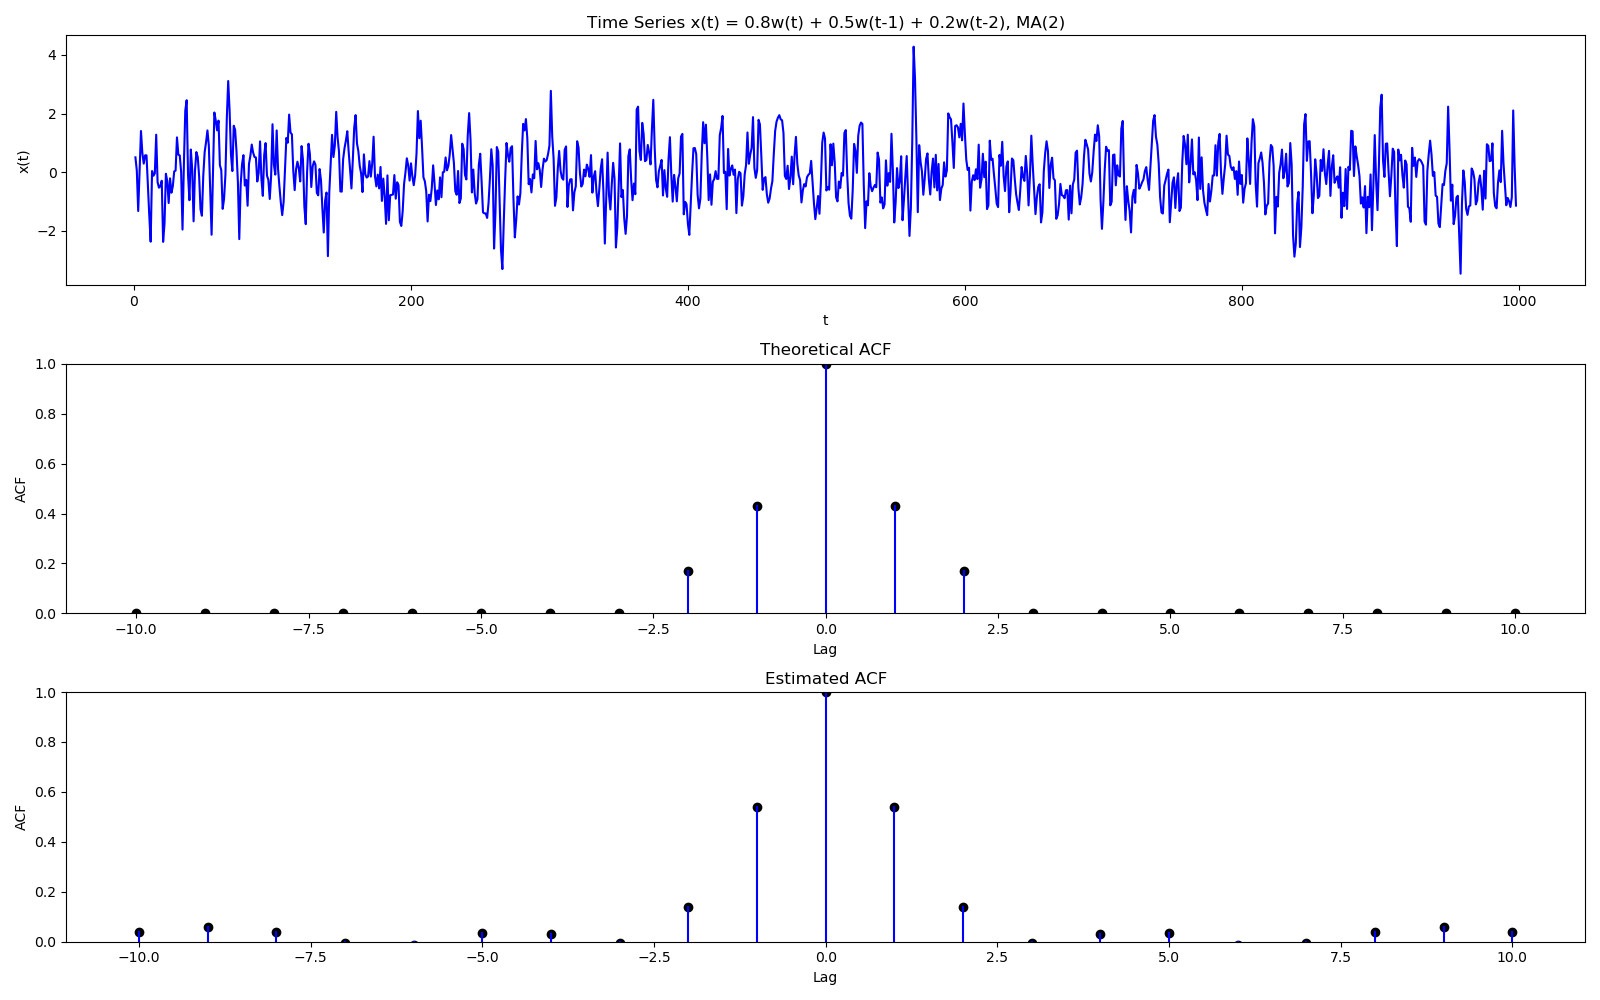
\includegraphics[scale=0.4]{acf_1}
    \centering
    \caption {Top figure shows a time series, with the theoretical and estimated ACFs shown by middle and bottom figures respectively. Due to the symmetric nature, most packages only plot ACF for positive lags. Figures plot using acf\_simulation.py}
    \label{fig:acf_1} %\ref{fig:acf_1}
\end{figure}
\end{document}